\chapter{Introduction}

\section{Metric space}

A metric $d$ on a set $X$, also called a distance function, is a function
that defines a distance between each pair of elements of the set. A
set with a metric is called a \textbf{metric space}.\\

Formally, $d : X \times X \rightarrow R$ is a metric if it is a function satisfying the following properties $\forall x, y, z \epsilon X$:
\begin{enumerate}
\item{Non-negativity : $d(x, y) \geq 0$}
\item{Indiscernability : $d(x, y) = 0$ iff $x = y$}
\item{Symmetry : $d(x, y) = d(y, x)$}
\item{Subadditivity : $d(x, y) + d(y, z) \geq d(x, z)$}
\end{enumerate}
\section{The Christofides' algorithm}
The Christofides' algorithm is an approximation algorithm for Metric TSP with an approximation ratio of $1.5$. Let G be a graph with $n$ points in the euclidean metric space. Below is a description of the steps involved in the Christofides' algorithm.
\vspace{0.7in}
\subsection{Pseudo code}
\textbf{Algorithm}
\begin{enumerate}
    \item{
        Find an MST of $G$, say $T$.        
    }
    \item {Compute a minimum cost perfect matching, $M$, on the set of odd-degree vertices of $T$.}
    \item {
        Add $M$ to $T$ and obtain an Eulerian multi-graph $H$.
    }
    \item {Find an Euler tour, $E$ of this graph.
    }
    \item {Output the tour that visits vertices of $G$ in order of their first appearance in $E$.}
\end{enumerate}
\begin{figure}[h]
    \centering
    \caption{MST $T$ of $G$}
    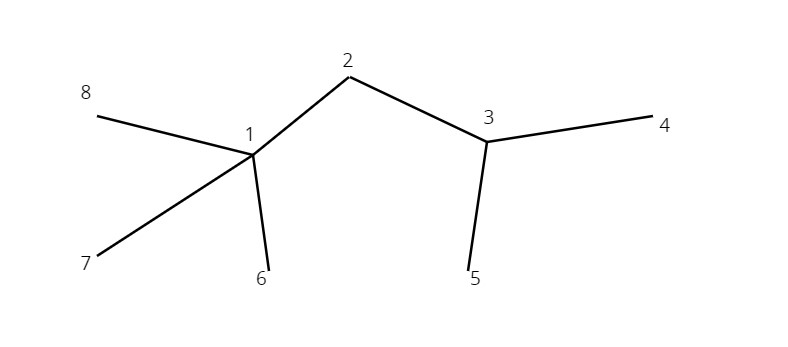
\includegraphics[scale=0.4]{1.jpg}
\end{figure}        
\begin{figure}[h]
    \centering
    \caption{Multi-graph $H$ of $G$}
    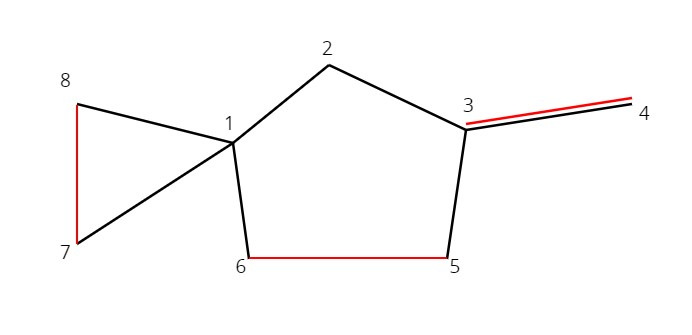
\includegraphics[scale=0.4]{2.jpg}
\end{figure}
\begin{figure}[h]
    \centering
    \caption{Euler tour $E$ of $H$}
    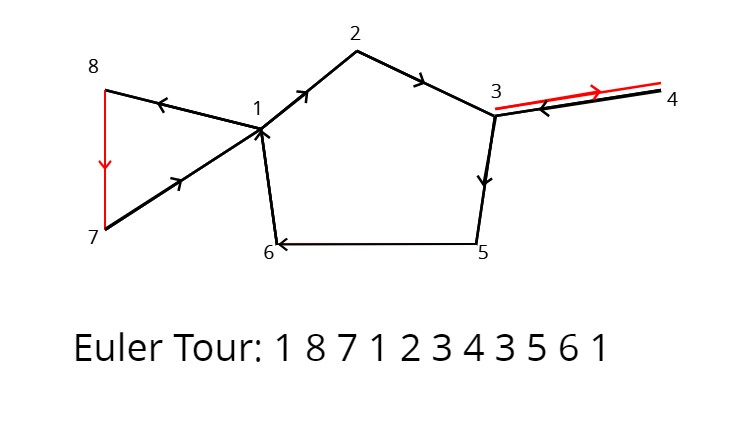
\includegraphics[scale=0.4]{3.jpg}
\end{figure}
\subsection{Time complexity}

some text\cite{citation-1-name-here}, some more texts

\subsubsection{<Sub-subsection title>}
even more text\footnote{<footnote here>}, and even more.

\section{Motivation}
